\section{Performance bounds}

Performance bounds offer valuable insights into the fundamental factors influencing the performance of a computer system. 
They can be computed swiftly and effortlessly, making them an ideal initial modeling technique.
Moreover, performance bounds allow for the simultaneous treatment of multiple alternatives, providing a comprehensive understanding of system performance.

\subsection{Bounding analysis}
Bounding analysis focuses on single-class systems and aims to establish asymptotic bounds, both upper and lower, on performance indices such as throughput ($X$) and response time ($R$). 
These bounds are viewed as functions of variables like the number of users or arrival rate.
By employing bounding analysis, critical influences of system bottlenecks can be highlighted and quantified, offering valuable insights into system performance.

\paragraph*{Bottleneck}
Bottleneck refers to the resource within a system that experiences the highest service demand, identified as $\max_k D_k$ where $D_k$ represents the service demand at each resource.
This resource, also known as the bottleneck device, plays a crucial role in limiting the overall performance of the system. 
Typically, the bottleneck resource exhibits the highest utilization within the system, making it a key determinant of system performance.

\paragraph*{Bounding analysis evaluation}
Bounding analysis offers several advantages. It effectively highlights and quantifies the critical influence of the system bottleneck, shedding light on the factors limiting system performance. 
Moreover, bounding analysis techniques can be computed swiftly, even by hand, making them accessible for quick assessments.
This approach proves especially useful in system sizing activities. 
It enables the evaluation of numerous candidate configurations, with a focus on the dominant resource, such as the CPU. 
By treating multiple configurations as a single alternative, bounding analysis streamlines decision-making based on preliminary estimates.

In terms of parameters and performance quantities, bounding analysis considers parameters such as the number of service centers ($K$), the sum of service demands at the centers ($D$), the largest service demand at any single center ($D_{\max}$), and the average think time for interactive systems ($Z$). 
Performance quantities of interest include the system throughput ($X$) and the system response time ($R$).

\subsection{Asymptotic bounds}
Asymptotic bounds are established by examining the extreme conditions of light and heavy loads, yielding both optimistic and pessimistic scenarios. 
These bounds provide insight into system performance under different operational conditions:
\begin{itemize}
    \item \textit{Optimistic bounds}: represent the upper limit for system throughput ($X$) and the lower limit for system response time ($R$).
    \item \textit{Pessimistic bounds}: represent the lower limit for system throughput ($X$) and the upper limit for system response time ($R$).
\end{itemize}
These bounds are determined under two extreme conditions: light load and heavy load. 
The analysis assumes that the service demand of a customer at a center remains consistent, irrespective of the number of other customers present in the system or their locations within the service centers.

\paragraph*{Open models asymptotic bounds}
In open models, where less information is available compared to closed models, asymptotic bounds provide insights into system behavior under varying conditions:
\begin{itemize}
    \item \textit{X bound}: represents the maximum arrival rate that the system can effectively process. 
        If the arrival rate $\lambda$ exceeds this bound, the system becomes saturated, leading to indefinite wait times for new jobs.
        The X bound $\lambda_{\text{sat}}$ is calculated as the reciprocal of the maximum service demand $D_{\max}$. 
    \item \textit{R bound}: Refer to the largest and smallest possible response times experienced at a given arrival rate $\lambda$. 
        These bounds are explored only when the arrival rate is less than the saturation arrival rate $\lambda_{\text{sat}}$, as the system becomes unstable otherwise.
        Two extreme situations are considered:
        \begin{enumerate}
            \item When no customers interfere with each other, resulting in response time $R$ equal to the sum of all service demands $(D=\sum_kD_k)$. 
            \item When there is no pessimistic bound on response times due to batch arrivals. 
                As the batch size $n$ increases, more customers wait increasingly longer times, leading to no pessimistic bound on response times regardless of how small the arrival rate $\lambda$ might be.
        \end{enumerate}
\end{itemize}
These bounds help evaluate system performance and stability under varying load conditions, providing crucial insights for system design and optimization.

\begin{figure}[H]
    \centering
    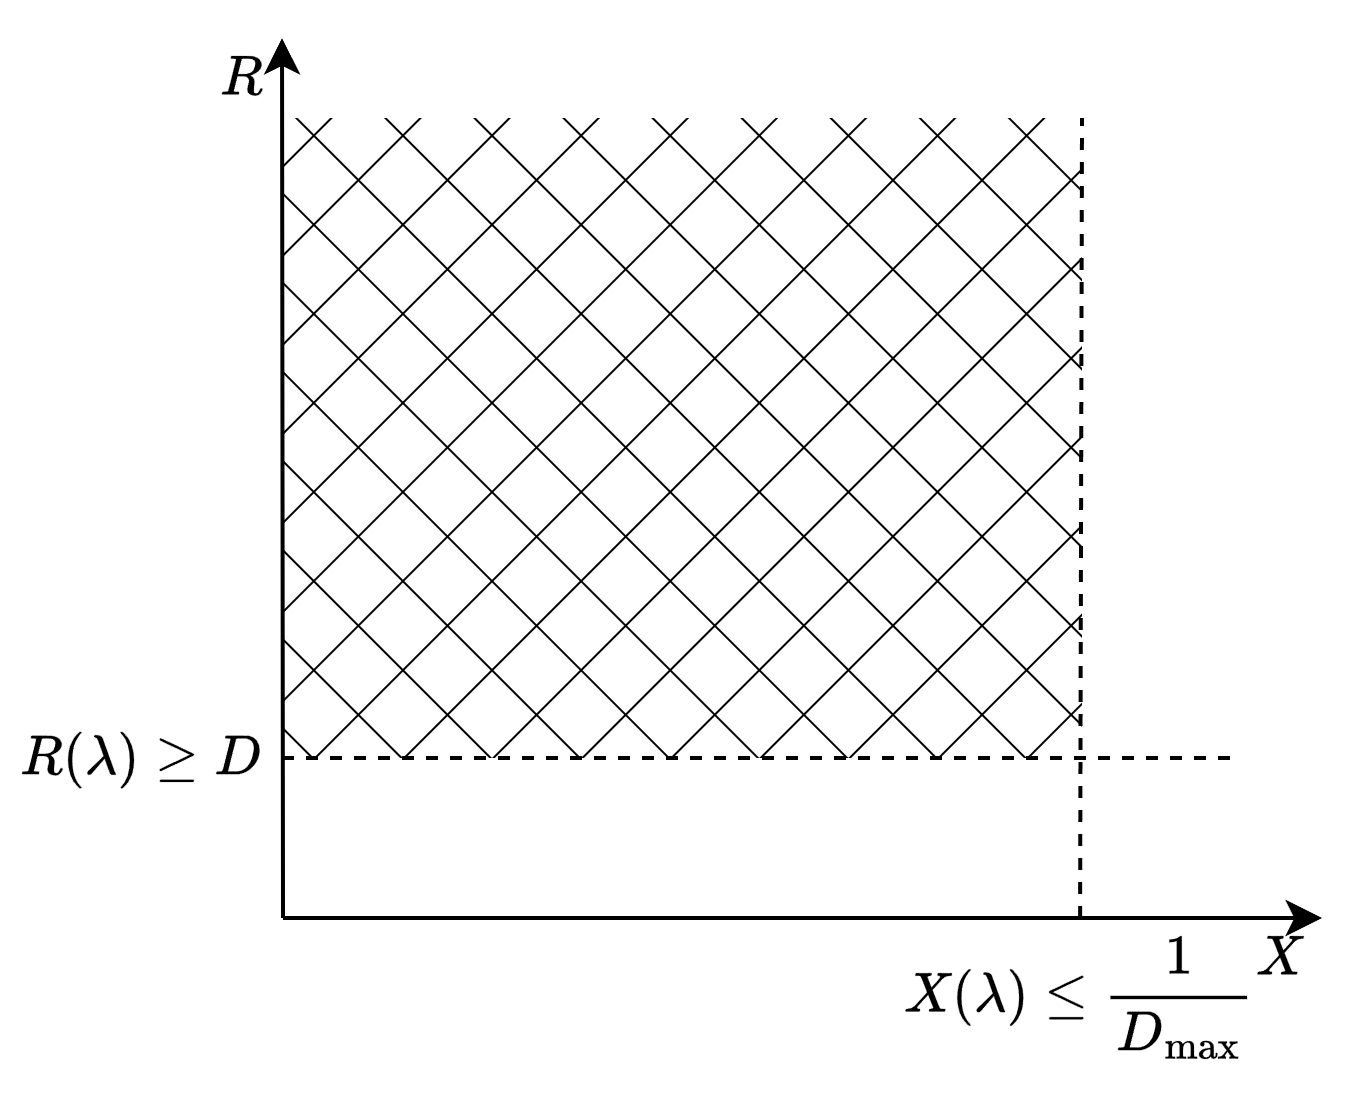
\includegraphics[width=0.45\linewidth]{images/cmod.png}
    \caption{Open loop asymptotic evaluation}
\end{figure}

\paragraph*{Closed models asymptotic bounds}
In closed models, we establish asymptotic bounds under both light and heavy load conditions to gain insights into system performance. 
Initially, we focus on determining bounds for system throughput $X$, which are then translated into bounds for system response time $R$ using Little's Law.
We have these following cases: 
\begin{itemize}
    \item \textit{Light load (lower bounds)}: With one customer in the system, the system throughput $X$ can be expressed as: 
        \[X=\dfrac{1}{D+Z}\]
        Here, $D$ represents the sum of service demands and $Z$ is the think time.

        As additional customers are added, the smallest $X$ is obtained when new jobs queue behind existing ones.
        This scenario results in: 
        \[X=\dfrac{N}{ND+Z}\]
        Here, $N$ is the total number of customers in the system.
        The limit of this expression approaches $X=\frac{1}{D}$ as $N$ increases.

        In closed models, the peak system response time arises when every job, at each station, encounters all the other $N-1$ customers ahead of it in the queue. 
    \item Light load (upper bounds): the largest $X$ is achieved when jobs consistently find the queue empty, and service begins immediately. 
        In this case: 
        \[X=\dfrac{N}{D+Z}\]
        The minimum response time is achieved when a job consistently encounters an empty queue and begins service immediately.
    \item Heavy load (upper bound): the system's utilization at each resource $U_k$ is constrained to be less than or equal to one. 
        Since the bottleneck resource is the first to saturate, $X(N)$ cannot exceed $\frac{1}{D_{\max}}$. 
        Thus, the bounds for $X(N)$ are: 
        \[\dfrac{N}{ND+Z}\leq X(N) \leq \min\left(\dfrac{1}{D_{\max},\frac{N}{D+Z}}\right)\]
        The parameter $N^\ast$ indicates the population size at which either the light or the heavy load optimistic bound is applied, determined by
        \[N^\ast=\dfrac{D+Z}{D_{\max}}\]

        Considering $X(N)=\frac{N}{(R(N)+Z)}$, the bounds for $R(N)$ are: 
        \[\dfrac{N}{ND+Z}\leq \dfrac{N}{R(N)+Z} \leq \min\left(\dfrac{1}{D_{\max},\frac{N}{D+Z}}\right)\]
        Consequently, the bounds for $R(N)$ are established as: 
        \[\max\left(D_{\max}-Z,D\right)\leq R(N) \leq ND\]
\end{itemize}

\subsection{What-if analysis}
What-if analysis is a decision-making technique used to explore the potential outcomes of various scenarios by changing one or more input variables in a model or system. 
It allows users to assess the impact of different decisions or changes by simulating how they would affect the results. 
By adjusting parameters and observing the resulting changes, decision-makers can gain insights into potential risks, opportunities, and optimal strategies. 